\documentclass[sigconf]{acmart}

\settopmatter{printacmref=false} % Removes citation information below abstract
\renewcommand\footnotetextcopyrightpermission[1]{} % removes footnote with conference information in first column
\pagestyle{plain} % removes running headers

\usepackage{booktabs} % For formal tables
\usepackage{hyperref}

\setcopyright{none} % Copyright

\newcommand{\rpm}{\raisebox{.2ex}{$\scriptstyle\pm$}}


\begin{document}

\title{OSX System Profiling}

\author{Rebecca McKinley}
\affiliation{%
  \institution{University of California, San Diego}
}
\email{rmckinle@eng.ucsd.edu}

\author{Daniel Reznikov}
\affiliation{%
  \institution{University of California, San Diego}
}
\email{drezniko@eng.ucsd.edu}


\author{Aaron Trefler}
\affiliation{%
  \institution{University of California, San Diego}
}
\email{atrefler@eng.ucsd.edu}

%%%%%%%%%%%%%%%%%%%%%%%%%%%%%%%%%%%%%%%
% Abstract
%%%%%%%%%%%%%%%%%%%%%%%%%%%%%%%%%%%%%%%
\begin{abstract}
The characteristic meta-challenge of profiling Computer Systems is the ability to isolate system components, control dependencies and optimizations, and to conduct well-defined, repeatable experimentation. The goal of this project is profile the OSX Operation System.
\end{abstract}

\maketitle

%%%%%%%%%%%%%%%%%%%%%%%%%%%%%%%%%%%%%%
% Introduction
%%%%%%%%%%%%%%%%%%%%%%%%%%%%%%%%%%%%%%
\section{Introduction}
We seek to measure the performance of our PC system components including CPU, RAM, disk and the network. We implement the supporting experimentation code in the language C as it is low-level enough to allow us to control for many system optimization, and at times to execute raw X86 Assembly instructions.

Our team members contribute equally to each part of the project. For each milestone, we would walk-through the design of each experiment together, and implement equal parts individually. We use Github for source control.


%%%%%%%%%%%%%%%%%%%%%%%%%%%%%%%%%%%%%%
% Machine Description
%%%%%%%%%%%%%%%%%%%%%%%%%%%%%%%%%%%%%%
\section{Machine Description} 
Using the command \textit{sysctl hw} and the \textit{System Information} OSX utility, we are able to identify the characteristic metrics of each system component which impacts our performance profiling. The specification summary is detailed in Table \ref{spec}.

\begin{table}[h!]
\centering
\caption{Machine Specification}
\label{spec}
\begin{tabular}{|l|l|}
\hline
\textbf{Component} & \textbf{Specification}                                                                                                     \\ \hline
CPU Model                 & Intel Core i7, 2.7 GHz, Dual Core                                                                                          \\ \hline
Cycle Time                & (1/2.7GHz) = 0.38ns                                                                                                        \\ \hline
L1 Cache                  & \begin{tabular}[c]{@{}l@{}}Instruction Cache: 32KB (per core) \\ Data Cache: 32KB (per core)\end{tabular}                  \\ \hline
L2 Cache                  & 256KB (per core) Level 2 Cache                                                                                             \\ \hline
L3 Cache                  & 6MB Total shared Level 3 Cache                                                                                             \\ \hline
RAM Size                  & 16GB (2 Banks of 8GB DDR3)                                                                                                 \\ \hline
Instruction Set           & x86-64                                                                                                                     \\ \hline
Memory Bus                & \begin{tabular}[c]{@{}l@{}}Type: DDR3\\ Speed: 1600MHz\\ Width: 64-bit\end{tabular}                                        \\ \hline
I/O Bus                   & \begin{tabular}[c]{@{}l@{}}Interconnect: SATA\\ Link Speed: 6 Gigabit\\ AHCI Version 1.30 Supported\end{tabular}           \\ \hline
Disk                      & \begin{tabular}[c]{@{}l@{}}Capacity: 500GB\\ Type: SSD\\ Mode: APPLE SSD SD512E\end{tabular}                               \\ \hline
Network Card              & \begin{tabular}[c]{@{}l@{}}Card Type: AirPort Extreme (0x14E4, 0xEF)\\ Firmware Version: Broadcom BCM43xx 1.0\end{tabular} \\ \hline
Operating System          & OSX 10.12                                                                                                                  \\ \hline
\end{tabular}
\end{table}



%%%%%%%%%%%%%%%%%%%%%%%%%%%%%%%%%%%%%%
% CPU Operations
%%%%%%%%%%%%%%%%%%%%%%%%%%%%%%%%%%%%%%
\section{CPU Operations}
\subsection{Read Time Overhead}
The x86 Instruction Set Architecture (ISA) supports an operation which allows the processor to increment the a register value at every clock cycle. It is well known that, having isolated environment optimizations as described in, a \textbf{\textit{rdtsc()}} method can be implemented in x86 assembly as follows:


\begin{figure}[h!]
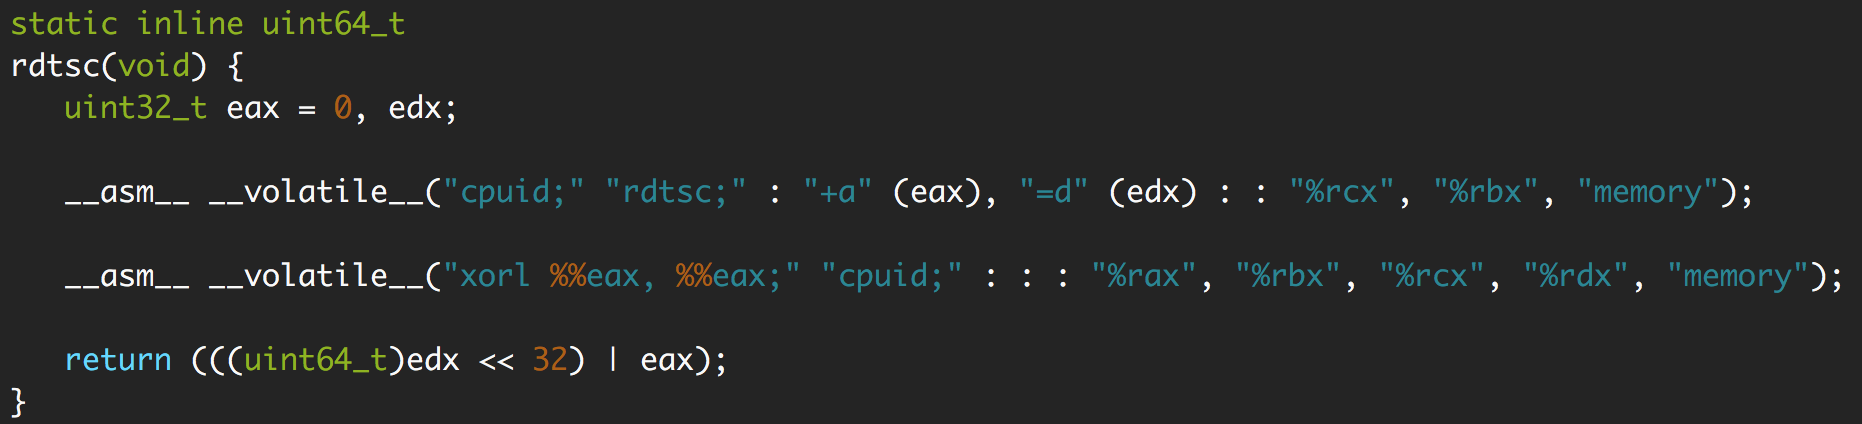
\includegraphics[scale=0.28]{images/rdtsc.png}
\end{figure}

%TODO reference env optimization turnoff handling.

% https://c9x.me/x86/html/file_module_x86_id_278.html
% https://www.intel.com/content/dam/www/public/us/en/documents/white-papers/ia-32-ia-64-benchmark-code-execution-paper.pdf

To profile the overhead of reading time, we execute an experiment which makes two consecutive calls to \textbf{\textit{rdtsc()}}, computes the number of elapsed cycles, and adds this to a running total which iterates this procedure 10M times. Aggregating over 10 experiment runs, we find the operation takes $avg(186) \rpm \sigma(5.34)$ cycles.

To profile the overhead of using a loop to measure many iterations of an operation, we 
orchestrate an experiment which executes an empty loop body 10M times, wrapping the loop in \textbf{\textit{rdtsc()}} calls. Aggregating over 10 experiment runs, we find that the overhead associated with a single loop iteration is $avg(5.4) \rpm \sigma(0.663325)$ cycles.

%%%%%%%%%%%%%%%%%%%%%%%%%%%%%%%%%%%%%%
% Conclusion
%%%%%%%%%%%%%%%%%%%%%%%%%%%%%%%%%%%%%%
\section{Conclusion}

%%%%%%%%%%%%%%%%%%%%%%%%%%%%%%%%%%%%%%
% Acknoweldgments
%%%%%%%%%%%%%%%%%%%%%%%%%%%%%%%%%%%%%%

\begin{acks}

\end{acks}
%%%%%%%%%%%%%%%%%%%%%%%%%%%%%%%%%%%%%%


\bibliographystyle{ACM-Reference-Format}
\bibliography{bibliography}

\end{document}
